\documentclass[11pt]{article}
%-----------Packeges---------------%
\usepackage{amsmath}
\usepackage{amssymb}
\usepackage{amsfonts}
\usepackage{tocloft}
\usepackage{float}
\usepackage{graphicx}
\usepackage[bookmarks=true]{hyperref}
\usepackage{fancyhdr}


%----------Definition & Theorem----%
\newtheorem{definition}{Definition}[subsection]
\newtheorem{theorem}{Theorem}[subsection]
\newtheorem{proposition}{Proposition}[subsection]
\newtheorem{lemma}{Lemma}[subsection]
\newtheorem{corollary}{Corollary}[subsection]

%\pagestyle{fancy}
%\fancyhead[L]{CS 412}
%\fancyhead[C]{Assignment 4}
%\fancyhead[R]{Lanxiao Bai}

\usepackage{listings}
\usepackage{color}
\usepackage{enumerate}
\usepackage{geometry}
\usepackage{longtable}
\geometry{left=2.5cm,right=2.5cm,top=2.5cm,bottom=2.5cm}

\definecolor{dkgreen}{rgb}{0,0.6,0}
\definecolor{gray}{rgb}{0.5,0.5,0.5}
\definecolor{mauve}{rgb}{0.58,0,0.82}

\lstset{frame=tb,
  language=Python,
  aboveskip=3mm,
  belowskip=3mm,
  showstringspaces=false,
  columns=flexible,
  basicstyle={\small\ttfamily},
  numbers=none,
  numberstyle=\tiny\color{gray},
  keywordstyle=\color{black},
  commentstyle=\color{dkgreen},
  stringstyle=\color{black},
  breaklines=true,
  breakatwhitespace=true,
  tabsize=3
}

\begin{document}
	\begin{center}
      \Large\textbf{CS 412 Assignment 4 Report}\\
      \large\textit{Lanxiao Bai}
   \end{center}
   
   \section{Introduction}
   \subsection{Decision Tree}
   \paragraph{}
    	Classification has long been a classic and important task of supervised learning. And for ordinary data, since it's not allowed to be compared by its magnitude, decision tree, in this case, is usually one of the best methods.
    	
    \paragraph{}
    	By recursively splitting datasets for training based on some attributes of the datasets, the decision tree algorithm can partition the input space $\mathcal{X}$ into different regions, so that the all (or at least majority of) points $x_i \in \mathcal{X}_j$ has the same label $y$.
    	
    \paragraph{}
    	In order to increase the purity of each branch after splitting, there're several evaluation metrics to determine based on which attribute and the corresponding value can the post-split purity reaches the highest value. In general, there're several properties that the impurity metric $\phi$ should meet in order to be use:
    	
    	For simplicity, we consider the metric for binary classification, and let $p$ be the probability of a label if uniformly randomly picked, then
    	
    	\begin{enumerate}
    		\item $\forall p \in [0, 1], \phi(1/2, 1/2) \geq \phi(p, 1 - p)$
    		\item $\phi(0, 1) = \phi(1, 0) = 0$
    		\item $p$ is increasing on $[0, 1/2]$ and decreasing on $[1/2, 1]$
    	\end{enumerate}
    
    \paragraph{}	
    	These properties and be easily extend to $k$-ary classification, and some of the most commonly used methods are
    	\begin{itemize}
    		\item Entropy: $\phi(p) = -(p\log_2p + (1 - p)\log_2(1 - p))$
    		\item Gini index: $\phi(p) = 2p(1 - p)$
    	\end{itemize}
    	
    \paragraph{}
    	In the experiment, the $k$-ary Gini index 
    	
    	\[\phi(\mathbf{p}) = 1 - \sum_{p_i \in \mathbf{p}} p_i^2\]
    	is used to measure the performance of splits by each attribute.
    	
    \paragraph{}
    	Since decision tree suffers greatly from overfitting and thus generalize not well, we applied the following strategies to reduce the generalize error
    	
    	\begin{itemize}
    		\item Set the maximum height $h$ that a tree can grow
    		\item Set the minimum Gini gain required to grow a node
    	\end{itemize}
    	
    \subsection{Random Forest}
    \paragraph{}
    	In order to reduce the variance of the model, we applied random forest algorithm. By uniformly sampling data from training dataset with replacement and randomly choosing $f$ attributes for a node to pick and grow, we made use of bagging strategy to randomize the training process. And other details of training algorithm we use is similar to the decision tree algorithm.
    
    \paragraph{}
    	Theoretically speaking, as the number of trees we use in the tree grows, the model will converge greatly, and the phenomenon of overfitting will also be mitigated by majority vote of the trees we train.
    	
    \subsection{Evaluation}
    \paragraph{}
    	Since it is possible that a node in the tree has unseen values or unseen features, in order that every data can be predicted as accurately as possible, I applied the strategy that in each node in the tree, we stored the majority label in the training dataset remaining, so that if a value or feature is unseen, we can use the majority vote the determine the prediction to be returned.
    	
    \section{Experiment}
    \paragraph{}
    To test our models, we ran our algorithm on four datasets: \textit{balance.scale}, \textit{nursery}, \textit{led} and \textit{synthetic.social}.
    
    \paragraph{}
    For simplicity, we fixed the Gini gain tolerance $\tau = 0.01$ and use the best depth for decision tree and best number of trees for random forest(which are explained later in Section 3).
    
    And our results are as following:
    \begin{center}
    \begin{longtable}{| c | c | c | c | c | c | c | c | c | c |}
    		\hline
    		 & & Overall Accuracy & Accuracy & Specificity & Precision & Recall & $F_1$ & $F_{0.5}$ & $F_2$\\
    		 \hline
    		 \textit{balance} & 1 &  & 1.0 & 1.0 & 1.0& 1.0& 1.0& 1.0& 1.0\\
    		                  & 2 & 1.000 & 1.0 & 1.0 & 1.0& 1.0& 1.0& 1.0& 1.0\\
    		 \textit{train}	  & 3 &  & 1.0 & 1.0 & 1.0& 1.0& 1.0& 1.0& 1.0\\
    		 \hline
    		 \textit{balance} & 1 &  & 0.805 & 0.892 & 0.0& 0.0& N/A& N/A & N/A\\
    		                  & 2 & 0.644 & 0.765 & 0.756 & 0.725 & 0.775 & 0.749 & 0.734 & 0.764\\
    		 \textit{test}	  & 3 &  & 0.72 & 0.774 & 0.702 & 0.653 & 0.677& 0.692 & 0.663\\
    		 \hline
    		                  & 1 & & 1.0 & 1.0 & 1.0& 1.0& 1.0& 1.0& 1.0\\
    		 \textit{nursery} & 2 & & 1.0 & 1.0 & 1.0& 1.0& 1.0& 1.0& 1.0\\
    		 \textit{train}	  & 3 & 1.000 & 1.0 & 1.0 & 1.0& 1.0& 1.0& 1.0& 1.0\\
    		                  & 4 & & 1.0 & 1.0 & 1.0& 1.0& 1.0& 1.0& 1.0\\
    		                  & 5 & & 1.0 & 1.0 & 1.0& 1.0& 1.0& 1.0& 1.0\\
    		 \hline
    		 				  & 1 & & 0.976 & 0.983 & 0.965 & 0.961 & 0.963 & 0.964 & 0.961\\
    		 \textit{nursery} & 2 & & 0.985 & 0.991 & 0.706& 0.777& 0.74& 0.719& 0.762\\
    		 \textit{test}	  & 3 & 0.975 & 0.99 & 0.994 & 0.986& 0.98& 0.983& 0.985& 0.981\\
    		                  & 4 & & 1.0 & 1.0 & 1.0& 1.0& 1.0& 1.0& 1.0\\
    		                  & 5 & & 0.999 & 0.999 & 0.0& N/A& N/A& N/A& N/A\\
    		 \hline
    		 \textit{led}     & 1 & 0.860 & 0.86 & 0.899 & 0.77& 0.771& 0.77& 0.77& 0.771\\
    		 \textit{train}	  & 2 & & 0.86 & 0.771 & 0.899& 0.899& 0.899& 0.899& 0.899\\
    		 \hline
    		 \textit{led}     & 1 & 0.857&0.857 & 0.894 & 0.766& 0.775& 0.77& 0.768& 0.773\\
    		 \textit{test}    & 2 & & 0.857 & 0.775 & 0.899& 0.894& 0.896& 0.898& 0.895\\
    		 \hline
    		 \textit{synthetic} & 1 & & 0.962 & 0.966 & 0.899& 0.952& 0.925& 0.909& 0.941\\
    		                    & 2 & & 0.973 & 0.98 & 0.941& 0.951& 0.946& 0.943& 0.949\\
    		                    & 3 & 0.939 & 0.973 & 0.985 & 0.956& 0.936& 0.946& 0.952& 0.94\\
    		 \textit{train}	    & 4 & & 0.971 & 0.988 & 0.963& 0.918& 0.94& 0.954& 0.927\\
    		 \hline
    		 \textit{synthetic} & 1 & & 0.734 & 0.816 & 0.504& 0.511& 0.507& 0.505& 0.51\\
    		                    & 2 & & 0.737 & 0.841 & 0.459& 0.416& 0.436& 0.45& 0.424\\
    		                    & 3 & 0.501&0.772 & 0.837 & 0.508& 0.556& 0.531& 0.517& 0.546\\
    		 \textit{test}	    & 4 & &0.759 & 0.84 & 0.528& 0.522& 0.525& 0.527& 0.523\\
    		 \hline
    	\caption{Results from Decision Tree on Four Datasets}
    \end{longtable}
    \end{center}
    
    \begin{center}
    \begin{longtable}{| c | c | c | c | c | c | c | c | c | c |}
    		\hline
    		 & & Overall Accuracy & Accuracy & Specificity & Precision & Recall & $F_1$ & $F_{0.5}$ & $F_2$\\
    		 \hline
    		 \textit{balance} & 1 &  & 0.955 & 1.0 & 1.0& 0.333& 0.5& 0.714& 0.384\\
    		                  & 2 & 0.945 & 0.968 & 0.958 & 0.953& 0.978& 0.965& 0.958& 0.973\\
    		 \textit{train}	  & 3 &  & 0.968 & 0.939 & 0.935& 1.0& 0.966& 0.947& 0.986\\
    		 \hline
    		 \textit{balance} & 1 &  & 0.898 & 0.995 & 0.0& 0.0& N/A& N/A& N/A\\
    		                  & 2 & 0.729 & 0.778 & 0.797 & 0.755& 0.755& 0.755& 0.755& 0.755\\
    		 \textit{test}	  & 3 &  & 0.782 & 0.718 & 0.713& 0.861& 0.78& 0.738& 0.827\\
    		 \hline
    		                  & 1 & & 1.0 & 1.0 & 1.0& 1.0& 1.0& 1.0& 1.0\\
    		 \textit{nursery} & 2 & & 0.966 & 0.956 & 0.918& 0.985& 0.95& 0.931& 0.971\\
    		 \textit{train}	  & 3 & 0.966 & 0.977 & 1.0 & 0.929& 0.066& 0.123& 0.257& 0.081\\
    		                  & 4 & & 0.989 & 0.993 & 0.984& 0.98& 0.982& 0.983& 0.981\\
    		                  & 5 & & 1.0 & 1.0 & 1.0& 1.0& 1.0& 1.0& 1.0\\
    		 \hline
    		 				  & 1 & & 0.945 & 0.941 & 0.888& 0.951& 0.918& 0.9& 0.938\\
    		 \textit{nursery} & 2 & & 0.974 & 1.0 & 1.0& 0.015& 0.03& 0.071& 0.019\\
    		 \textit{test}	  & 3 & 0.939 & 0.971 & 0.977 & 0.95& 0.958& 0.954& 0.952& 0.956\\
    		                  & 4 & & 1.0 & 1.0 & 1.0& 1.0& 1.0& 1.0& 1.0\\
    		                  & 5 & & 1.0 & 1.0 & N/A& N/A& N/A& N/A& N/A\\
    		 \hline
    		 \textit{led}     & 1 & 0.841 & 0.841 & 0.937 & 0.814& 0.624& 0.706& 0.767& 0.655\\
    		 \textit{train}	  & 2 & & 0.841 & 0.624 & 0.85& 0.937& 0.891& 0.866& 0.918\\
    		 \hline
    		 \textit{led}     & 1 & 0.863&0.863 & 0.916 & 0.799& 0.746& 0.772& 0.788& 0.756\\
    		 \textit{test}    & 2 & & 0.863 & 0.746 & 0.89& 0.916& 0.903& 0.895& 0.911\\
    		 \hline
    		 \textit{synthetic} & 1 & & 1.0 & 1.0 & 1.0& 1.0& 1.0& 1.0& 1.0\\
    		                    & 2 & & 1.0 & 1.0 & 1.0& 1.0& 1.0& 1.0& 1.0\\
    		                    & 3 & 1.000 & 1.0 & 1.0 & 1.0& 1.0& 1.0& 1.0& 1.0\\
    		 \textit{train}	    & 4 & & 1.0 & 1.0 & 1.0& 1.0& 1.0& 1.0& 1.0\\
    		 \hline
    		 \textit{synthetic} & 1 & & 0.881 & 0.933 & 0.802& 0.739& 0.769& 0.789& 0.751\\
    		                    & 2 & & 0.879 & 0.936 & 0.782& 0.702& 0.74& 0.765& 0.717\\
    		                    & 3 & 0.775&0.9 & 0.926 & 0.768& 0.815& 0.791& 0.777& 0.805\\
    		 \textit{test}	    & 4 & &0.89 & 0.905 & 0.753& 0.847& 0.797& 0.77& 0.826\\
    		 \hline
    	\caption{Results from Random Forest Tree on Four Datasets}
    \end{longtable}
    \end{center}
    
    \section{Model Tuning}
    
    \paragraph{}
    
    The tuning principle is following:
    \begin{enumerate}
    	\item For Decision Tree, we fix the tolerance to $0$ and change the max depth of the tree
    	\item For Random forest, we fix data sample rate to $0.8$, feature sample number to the square root of the number of all features and change the number of trees in the forest
    \end{enumerate}
    
    \paragraph{}
    We got the following plots from the experiments above:
    \begin{figure}[H]
  		\begin{center}
  			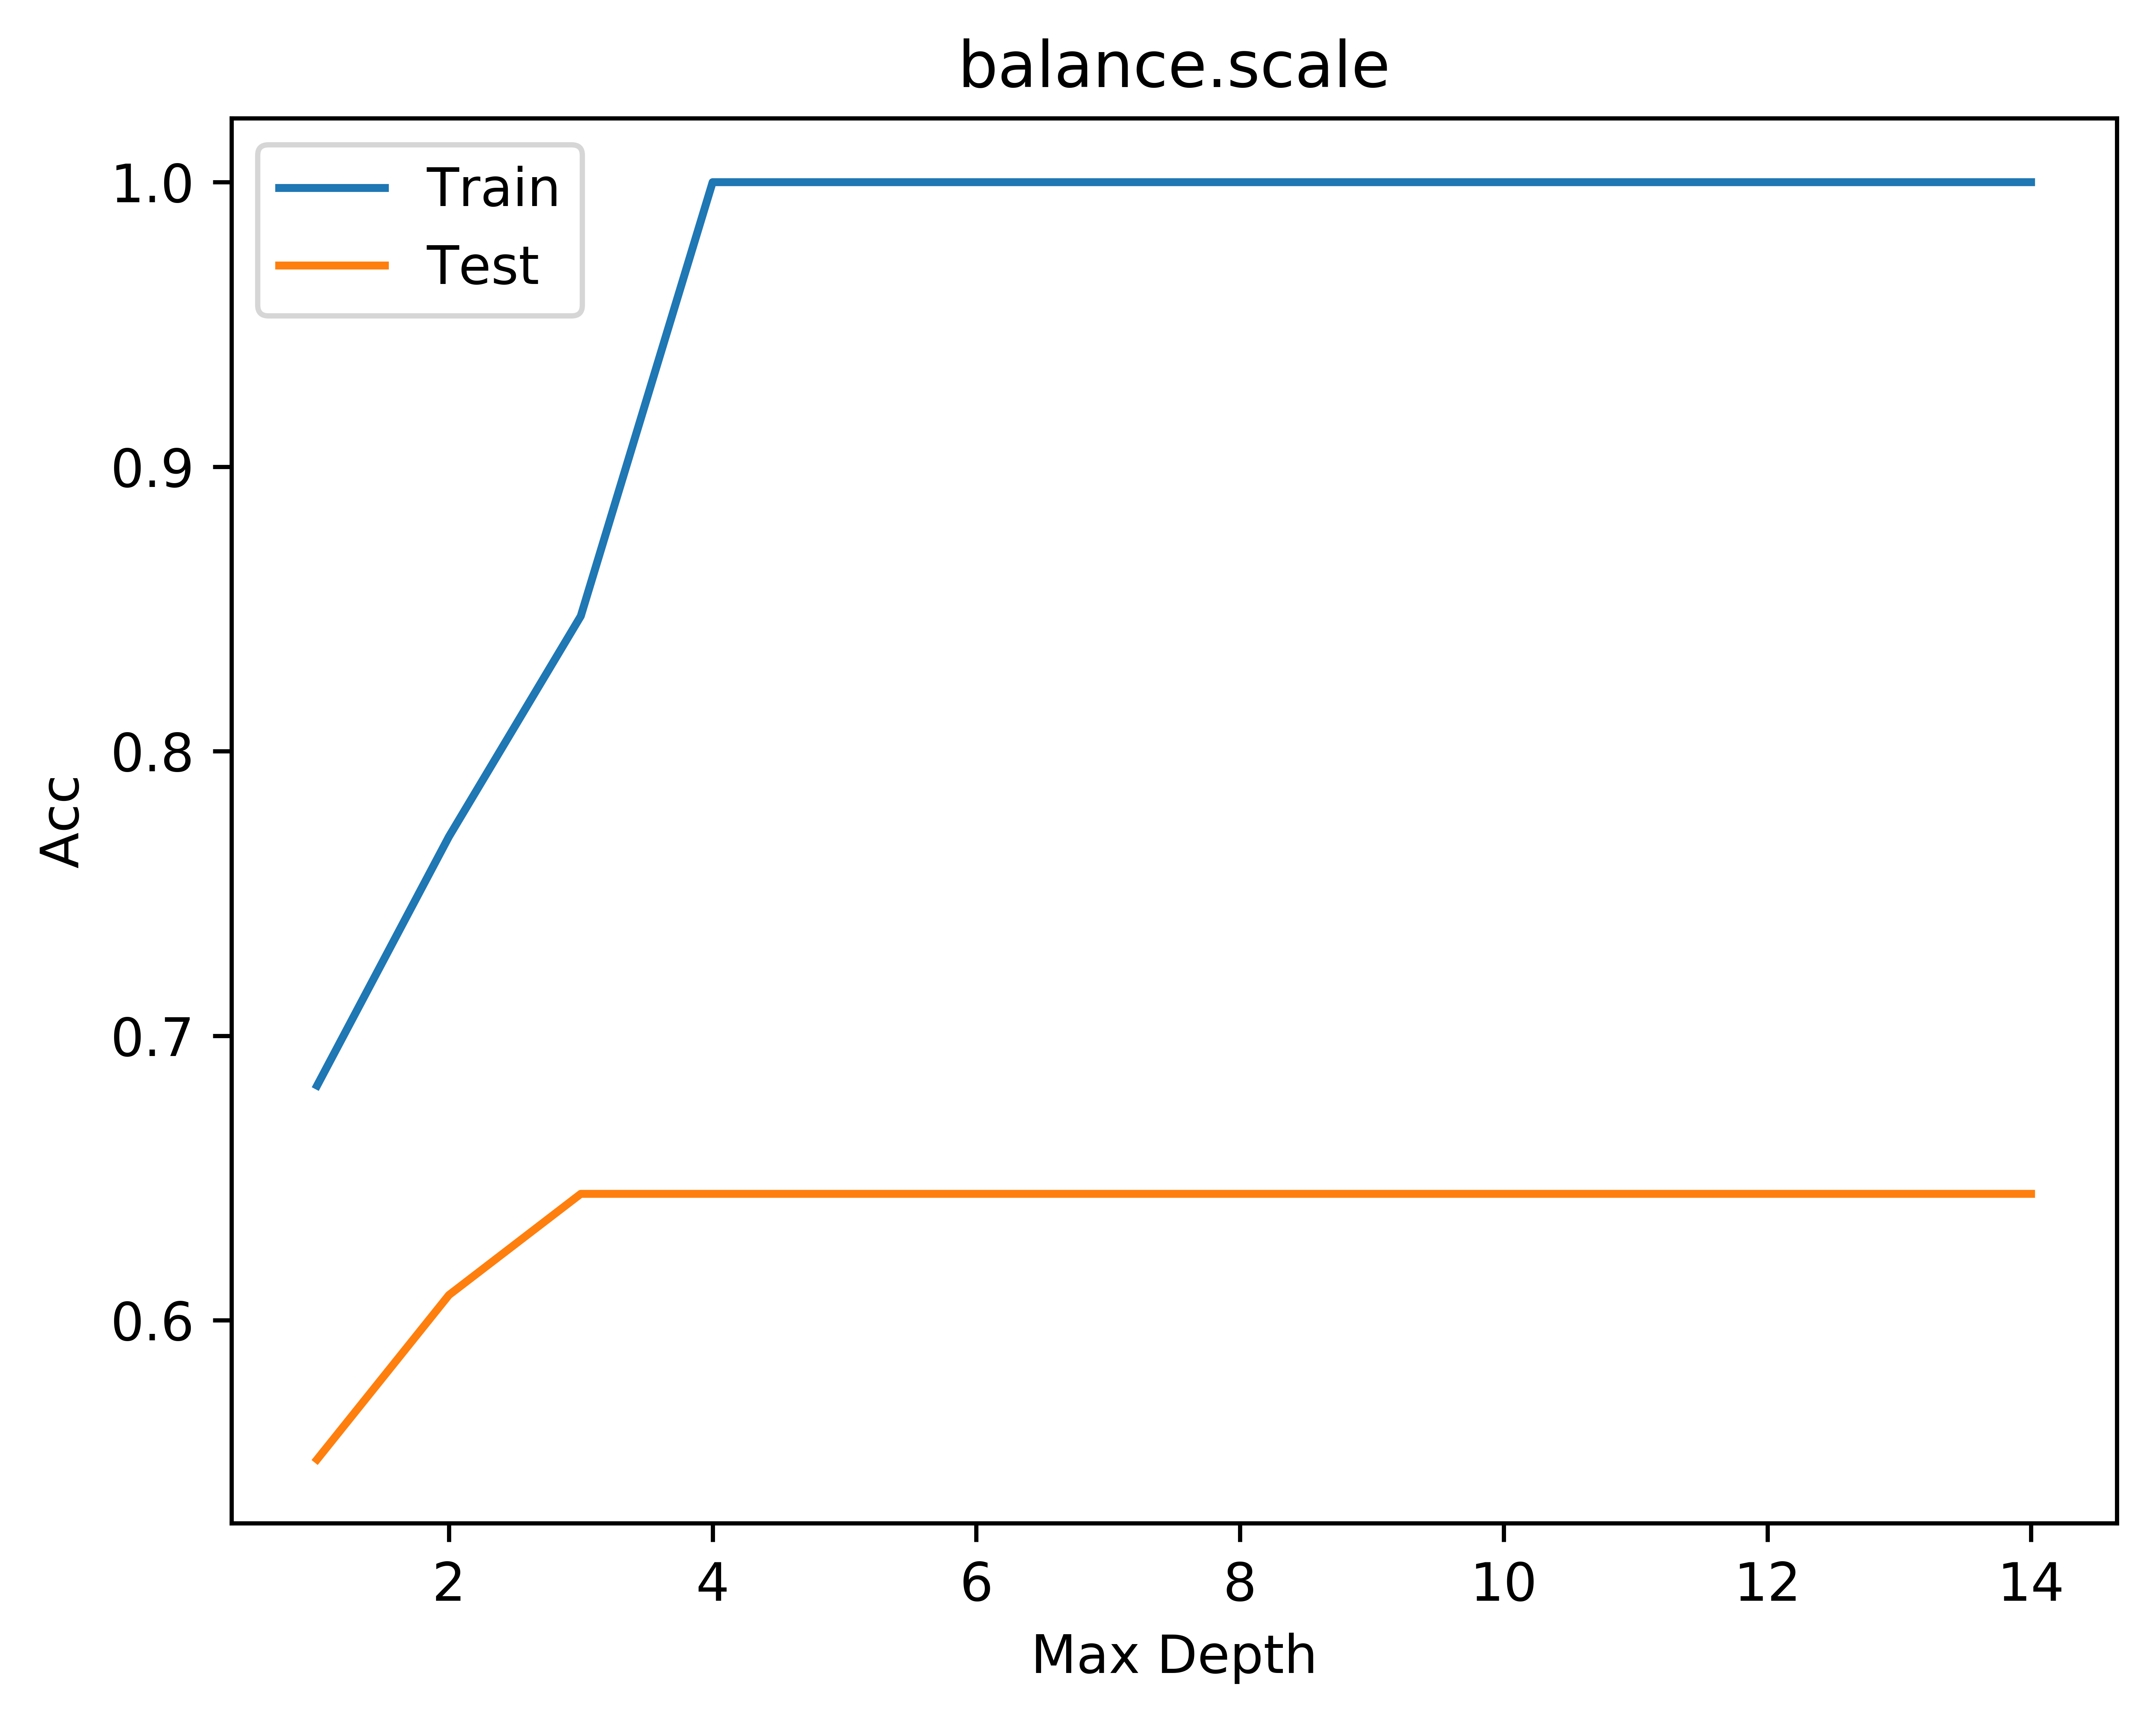
\includegraphics[width=8cm]{code/pics/balance_scale_DecisionTree}
  		\end{center}
	\end{figure}
	\begin{figure}[H]
  		\begin{center}
  			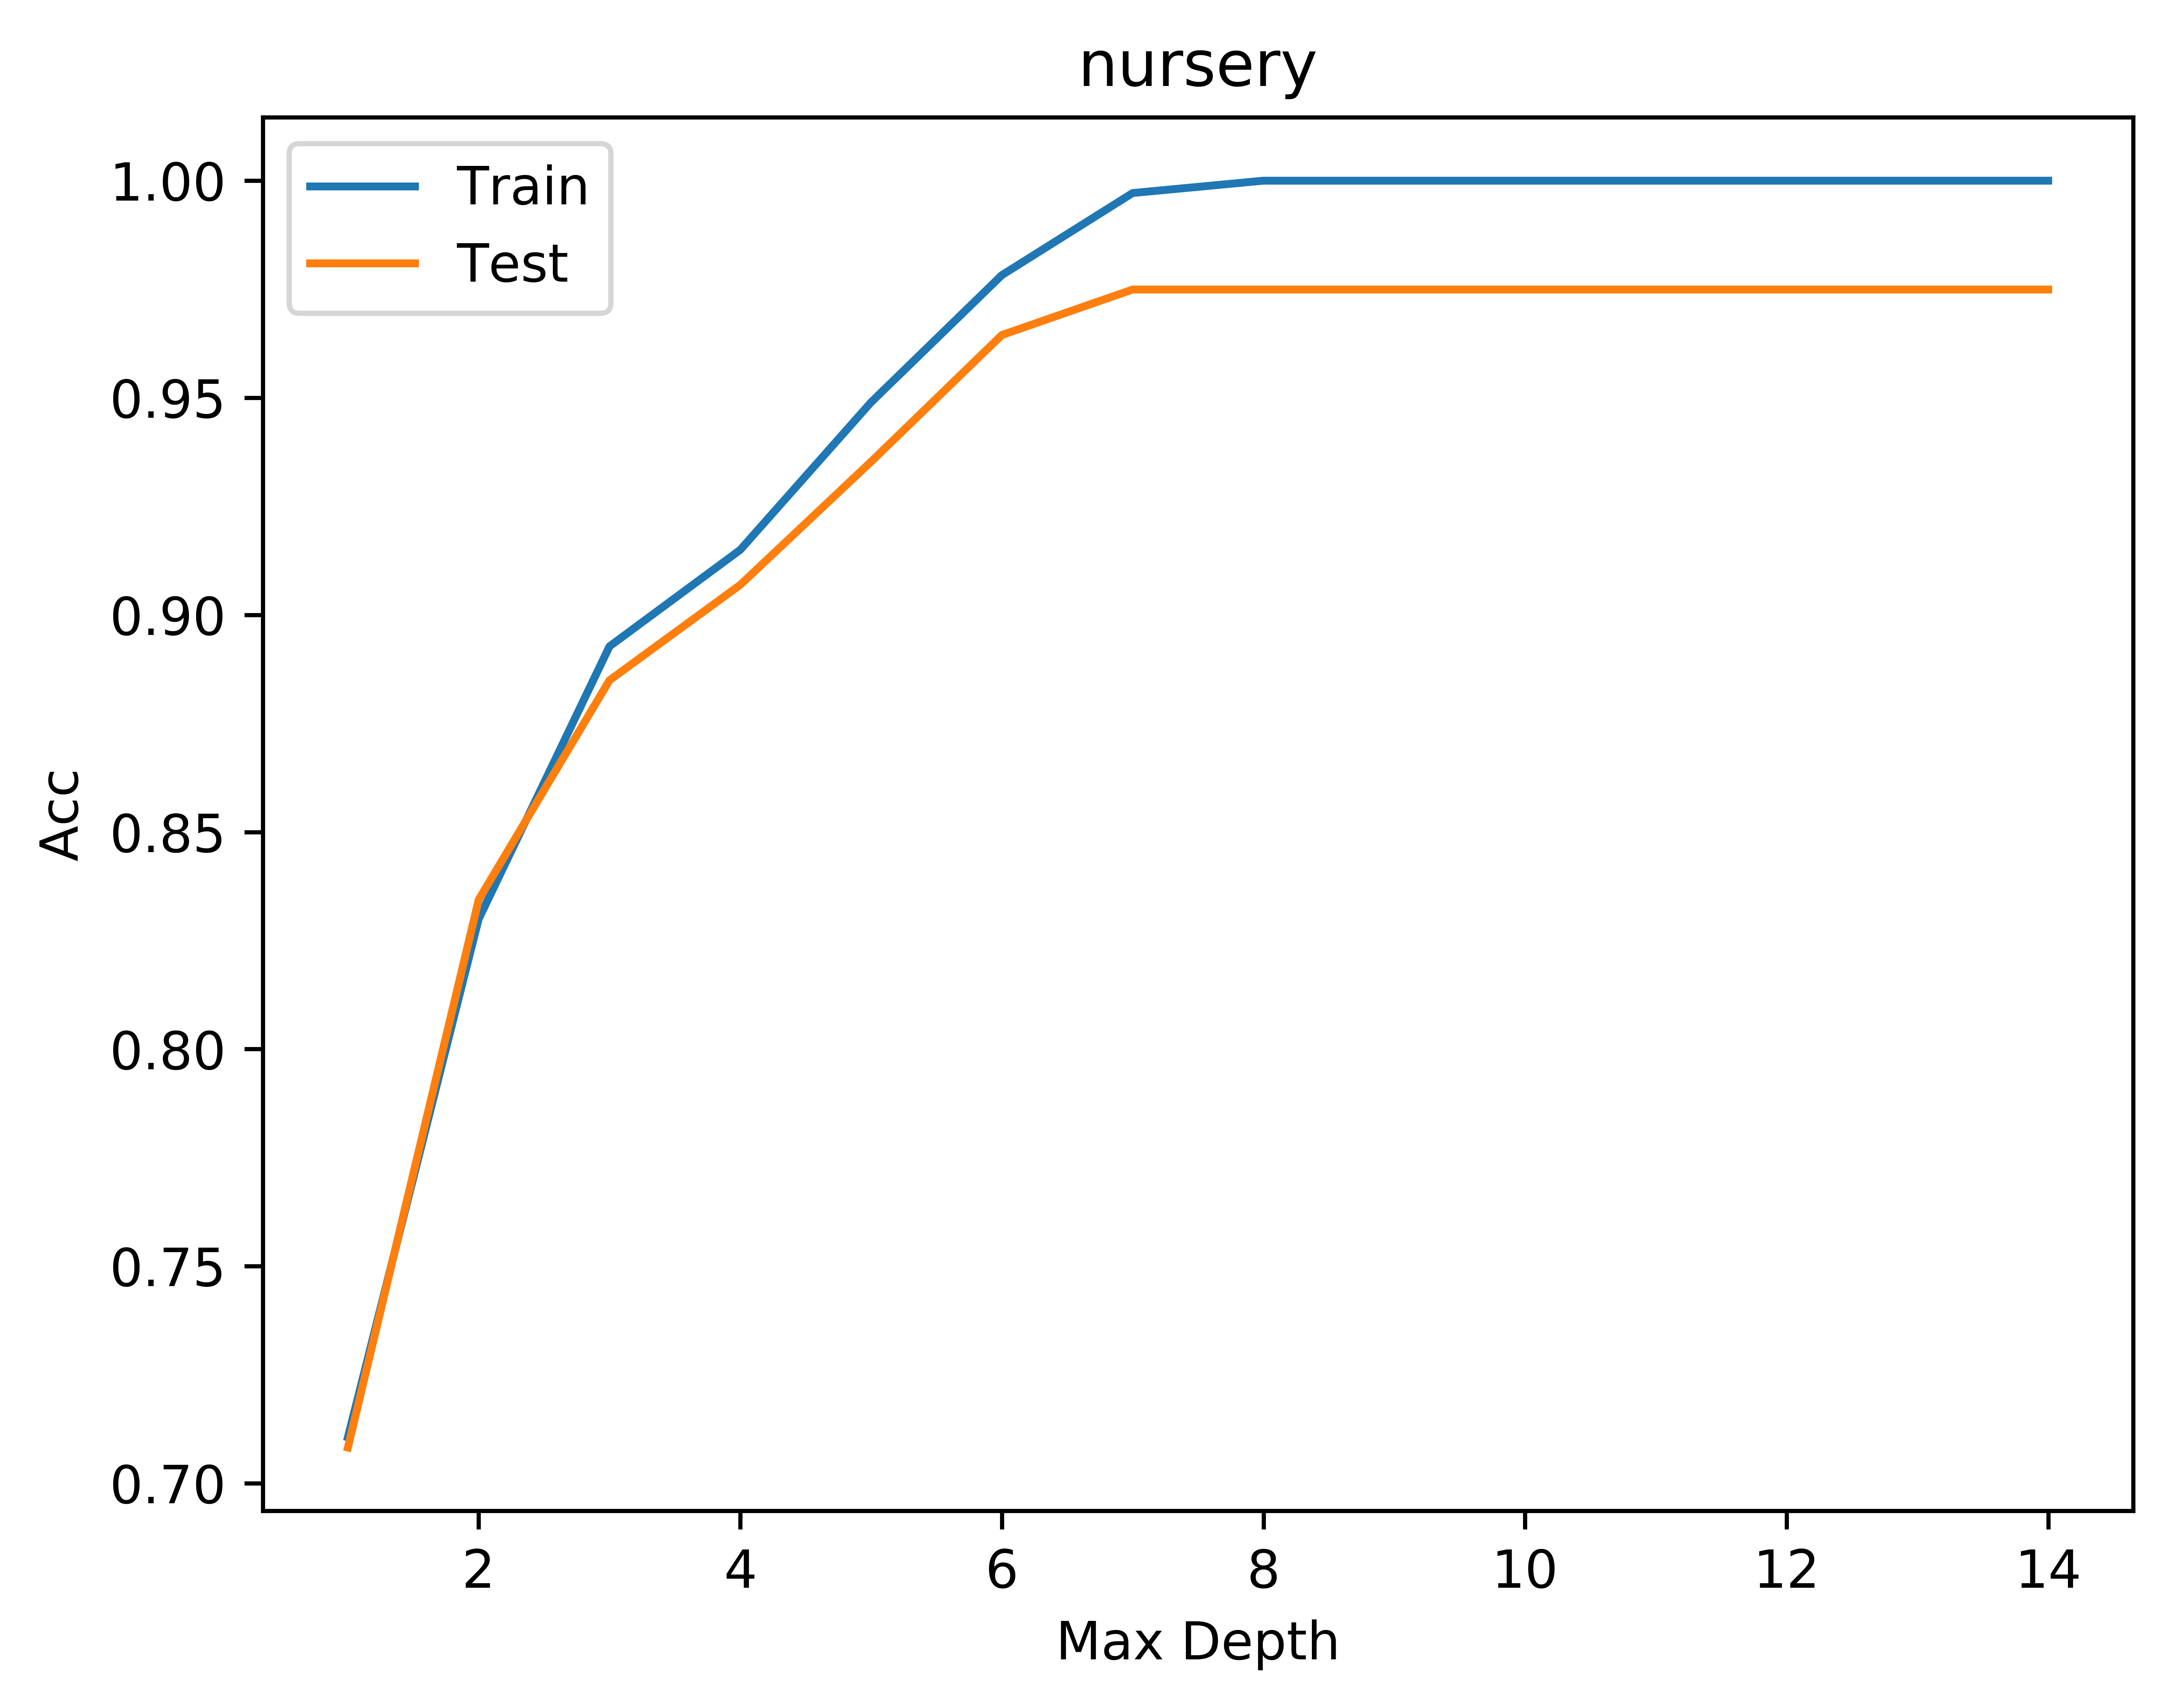
\includegraphics[width=8cm]{code/pics/nursery_DecisionTree}
  		\end{center}
	\end{figure}
	\begin{figure}[H]
  		\begin{center}
  			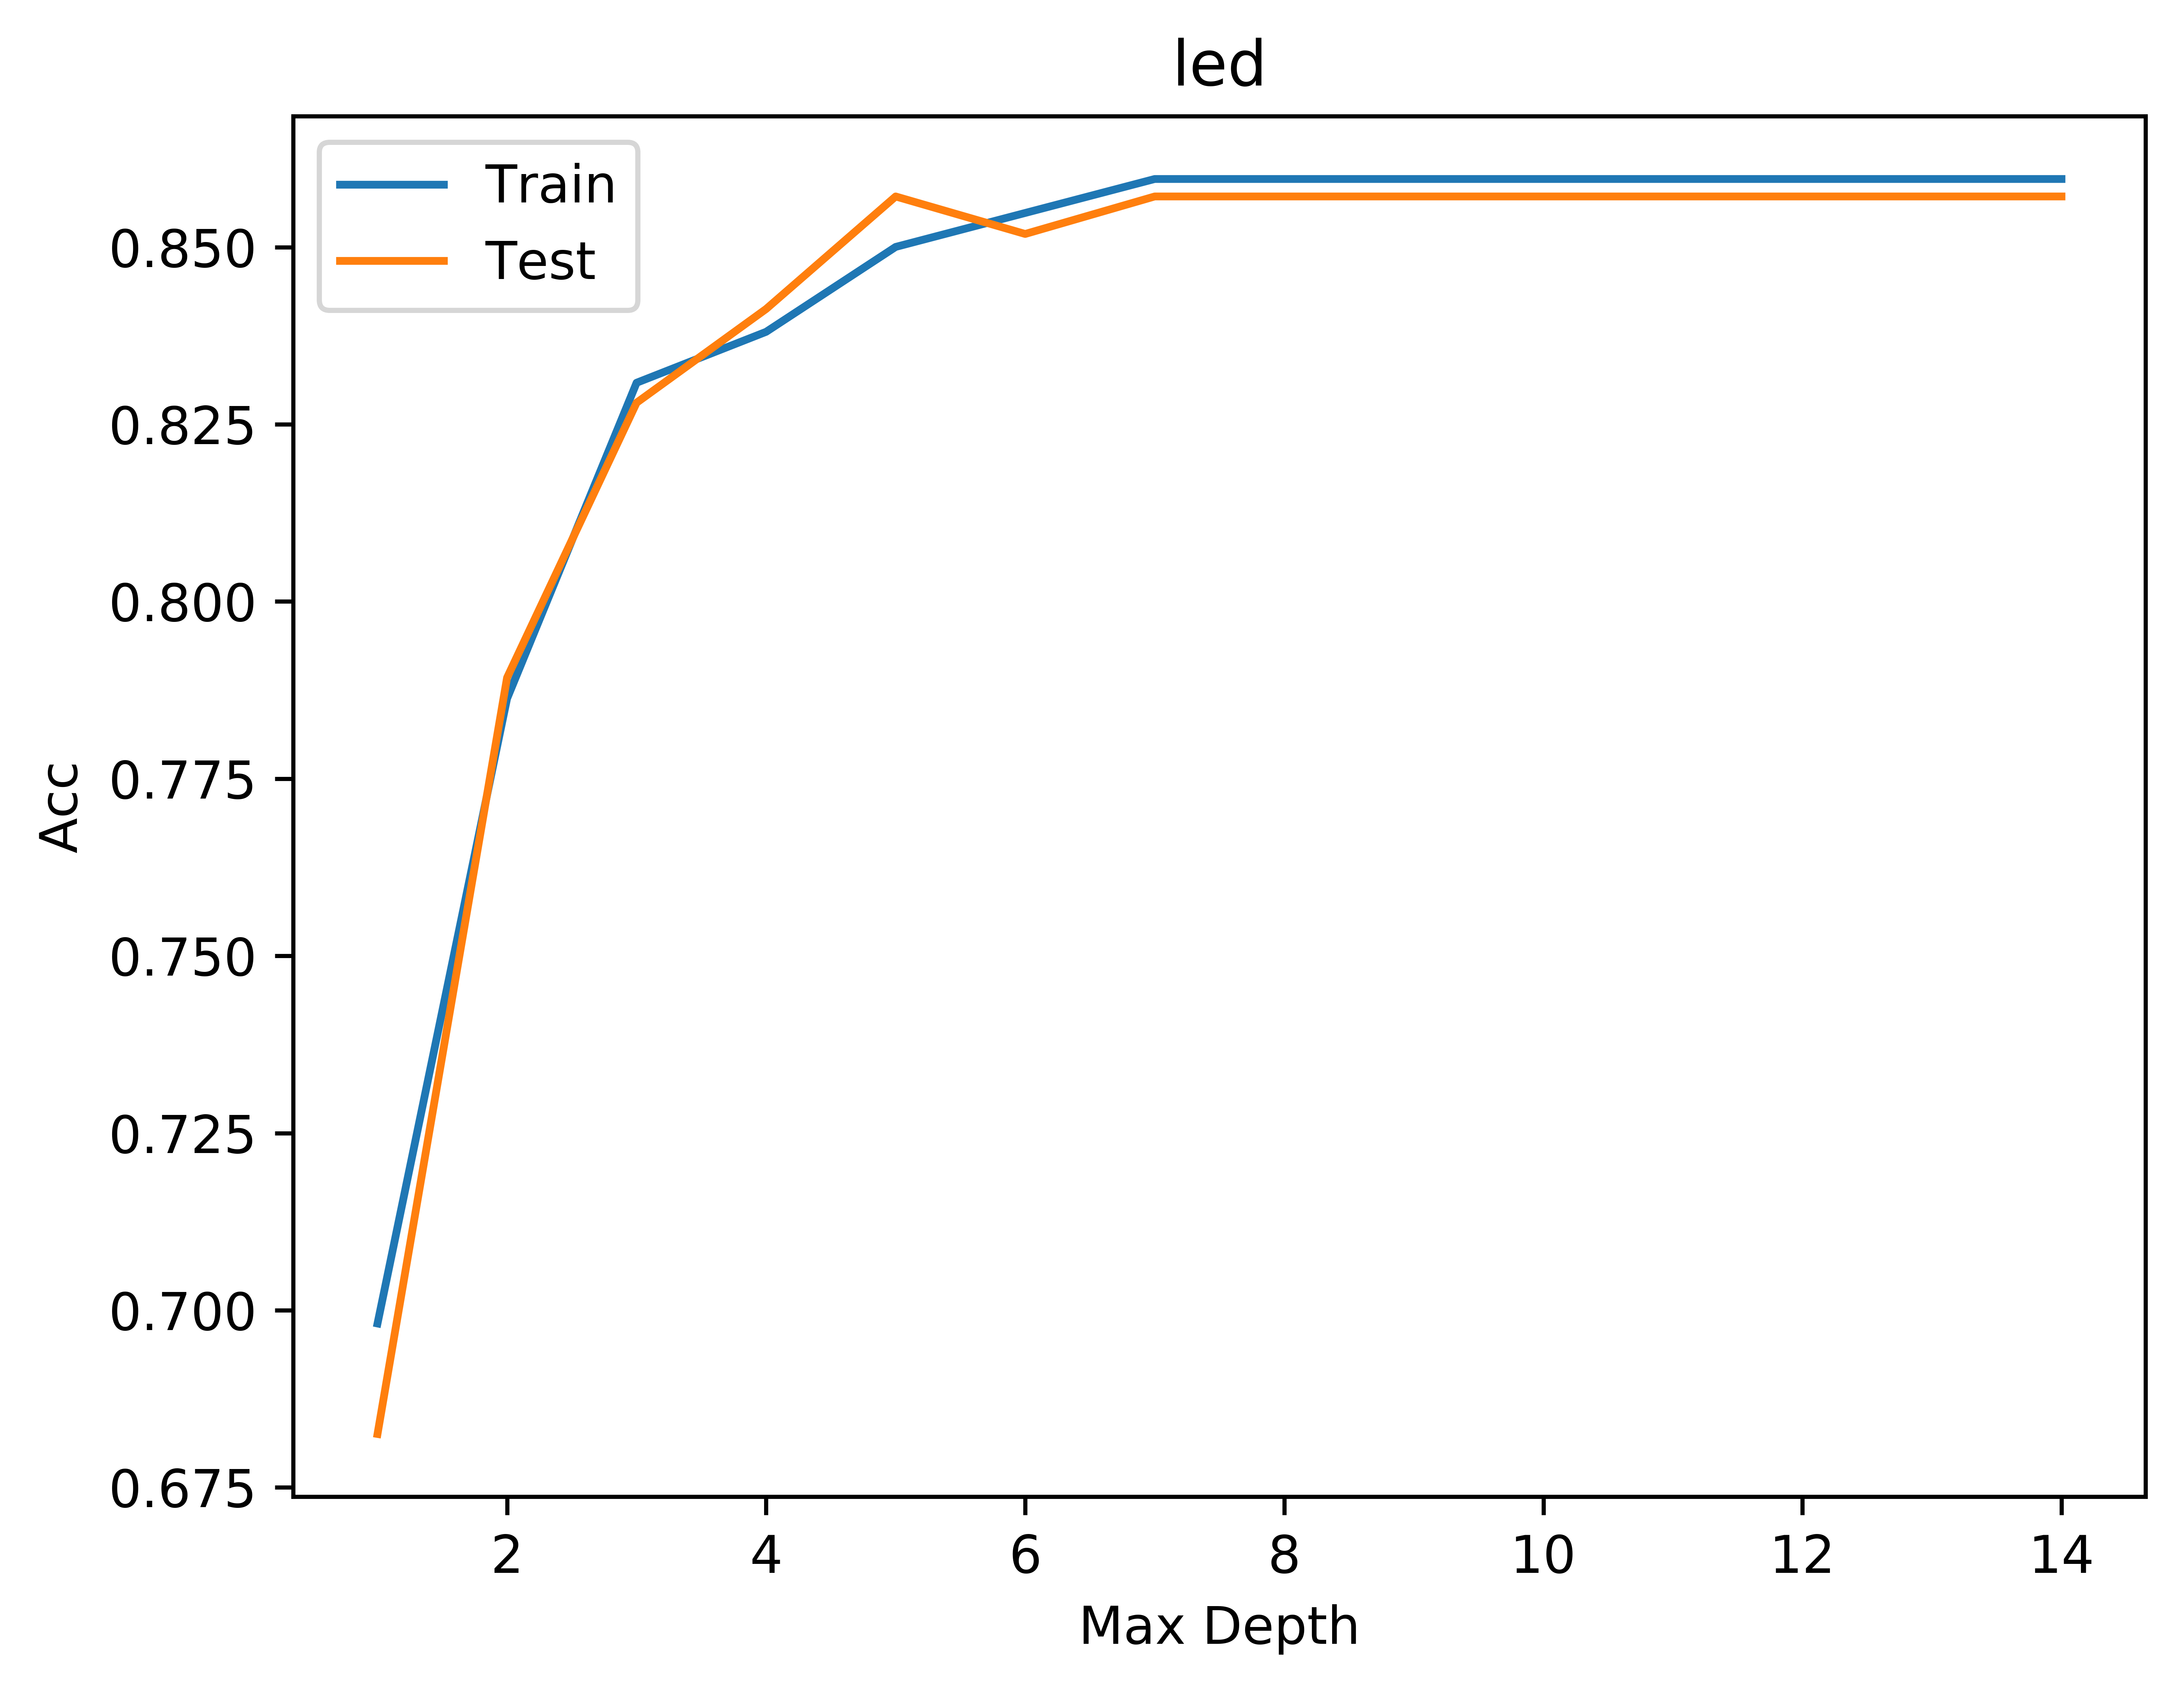
\includegraphics[width=8cm]{code/pics/led_DecisionTree}
  		\end{center}
	\end{figure}
	\begin{figure}[H]
  		\begin{center}
  			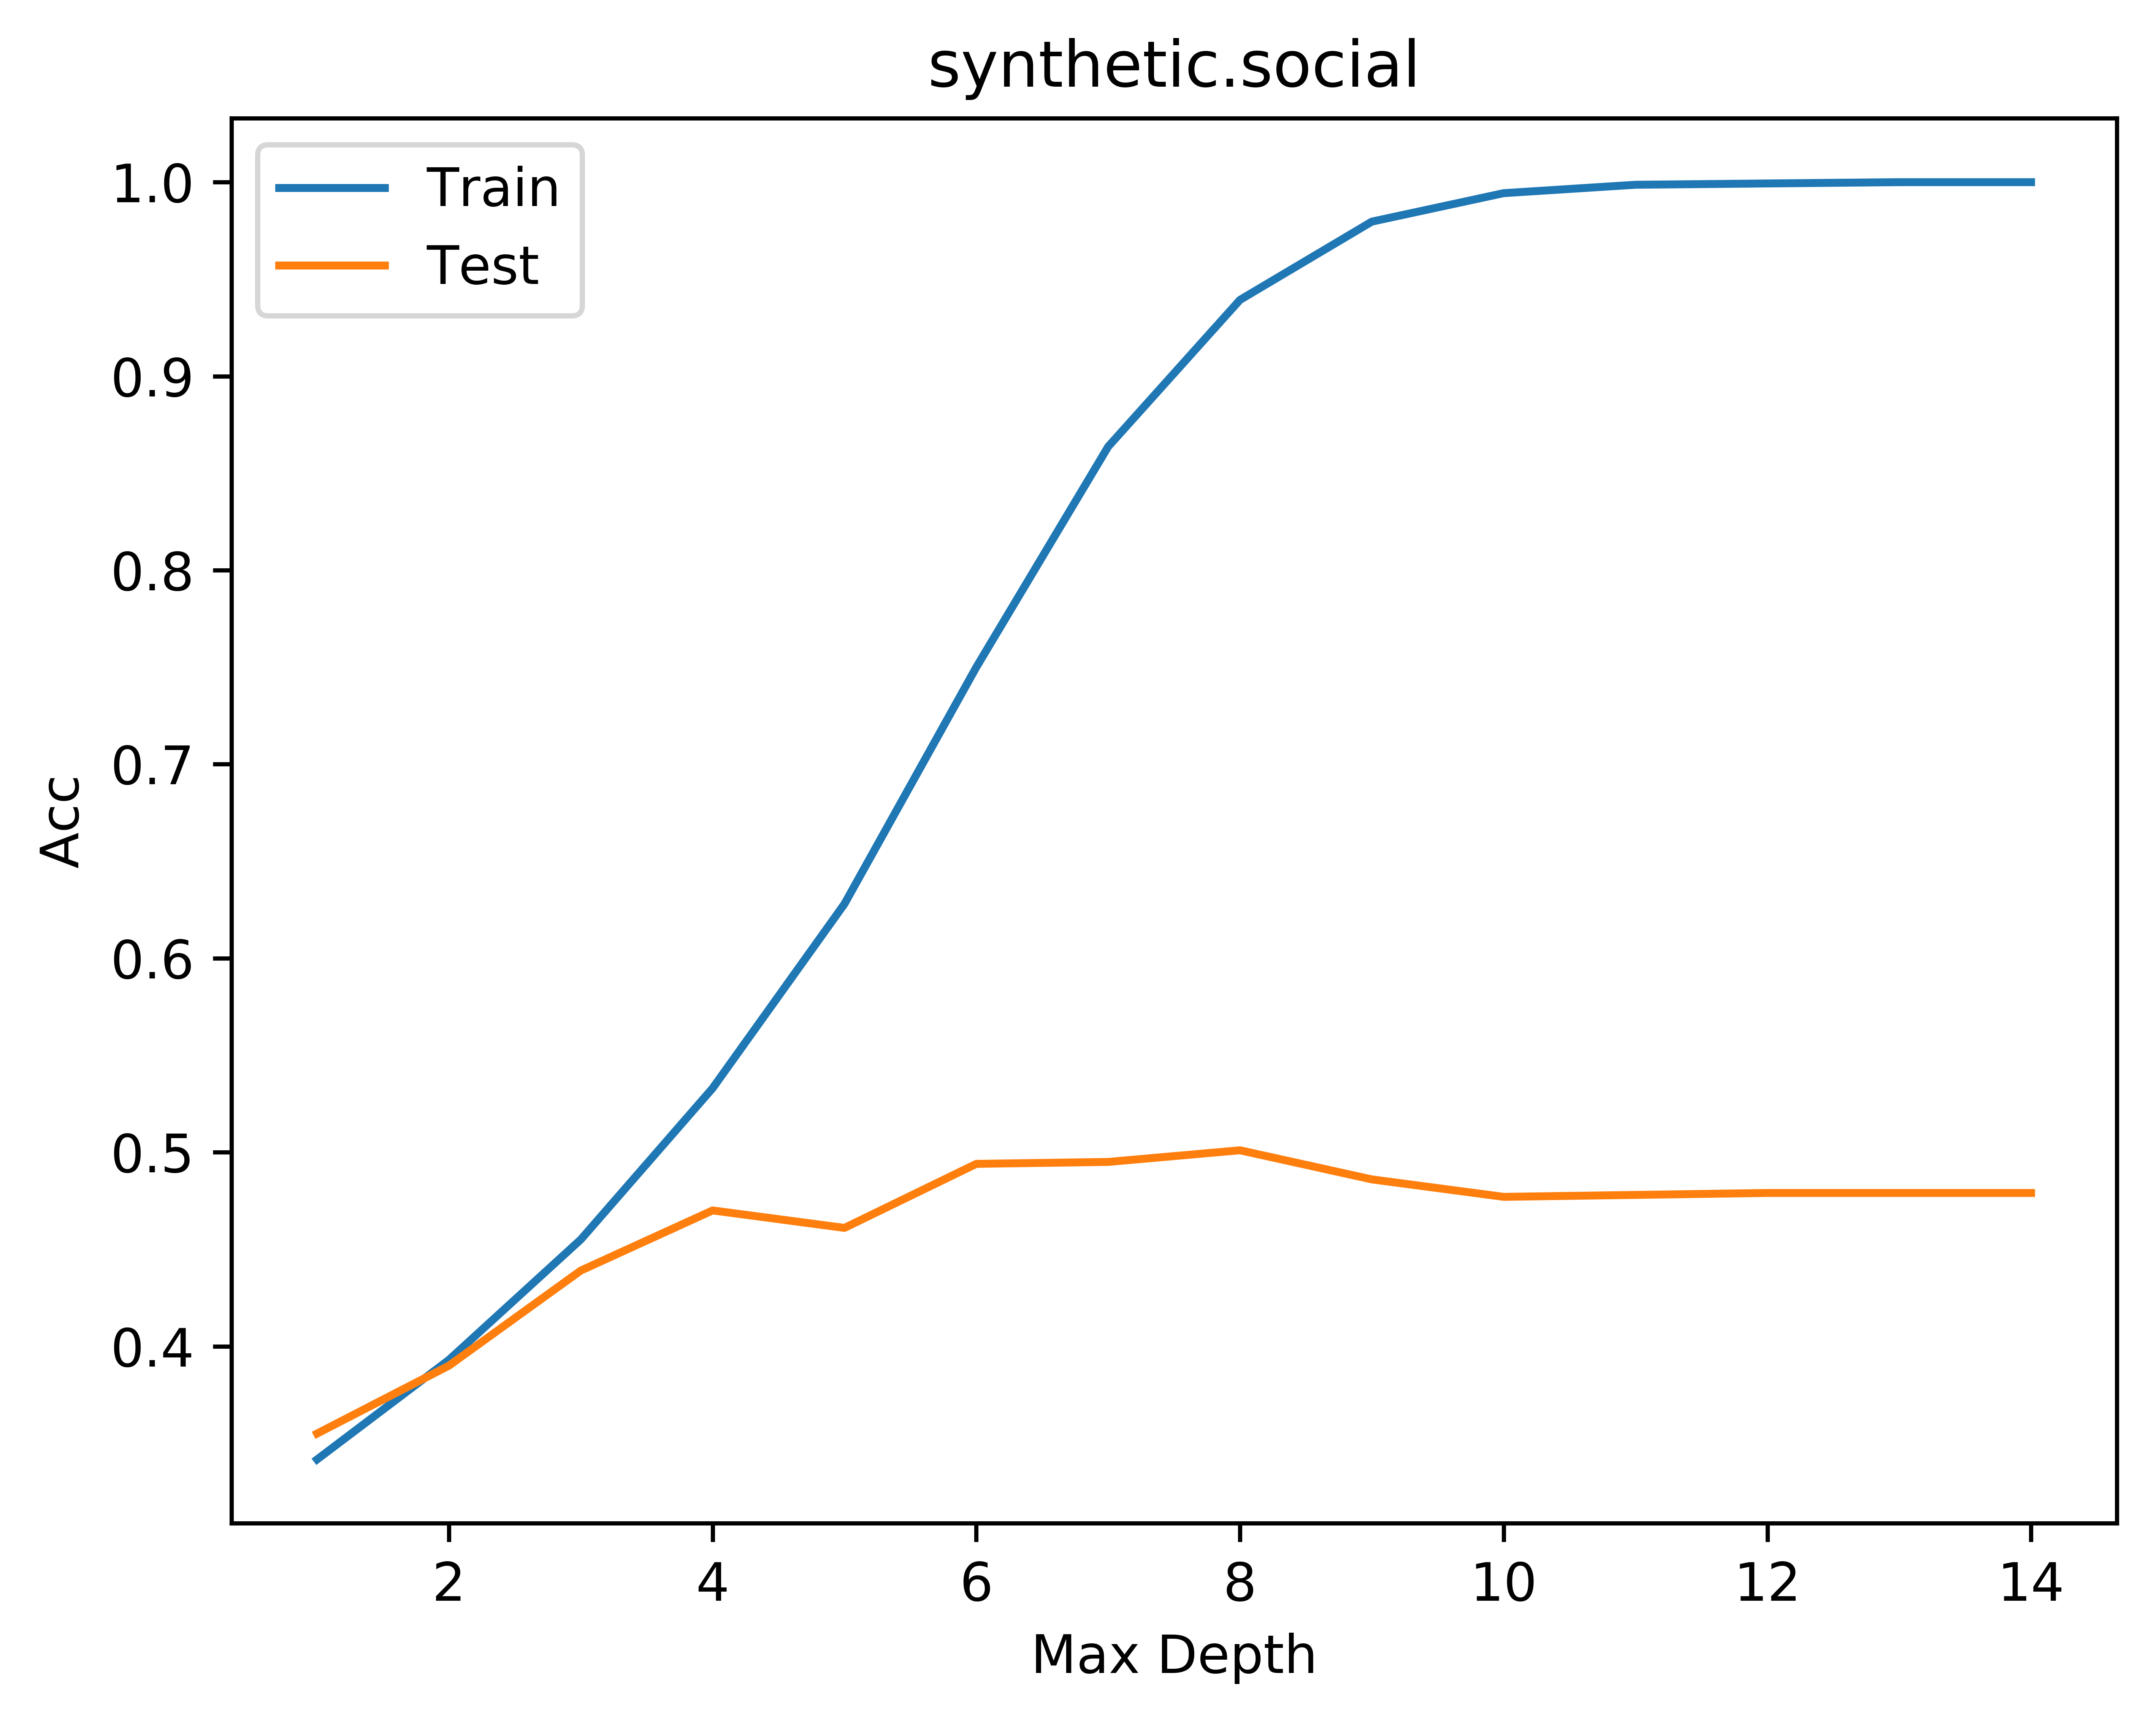
\includegraphics[width=8cm]{code/pics/synthetic_social_DecisionTree}
  		\end{center}
	\end{figure}
	\begin{figure}[H]
  		\begin{center}
  			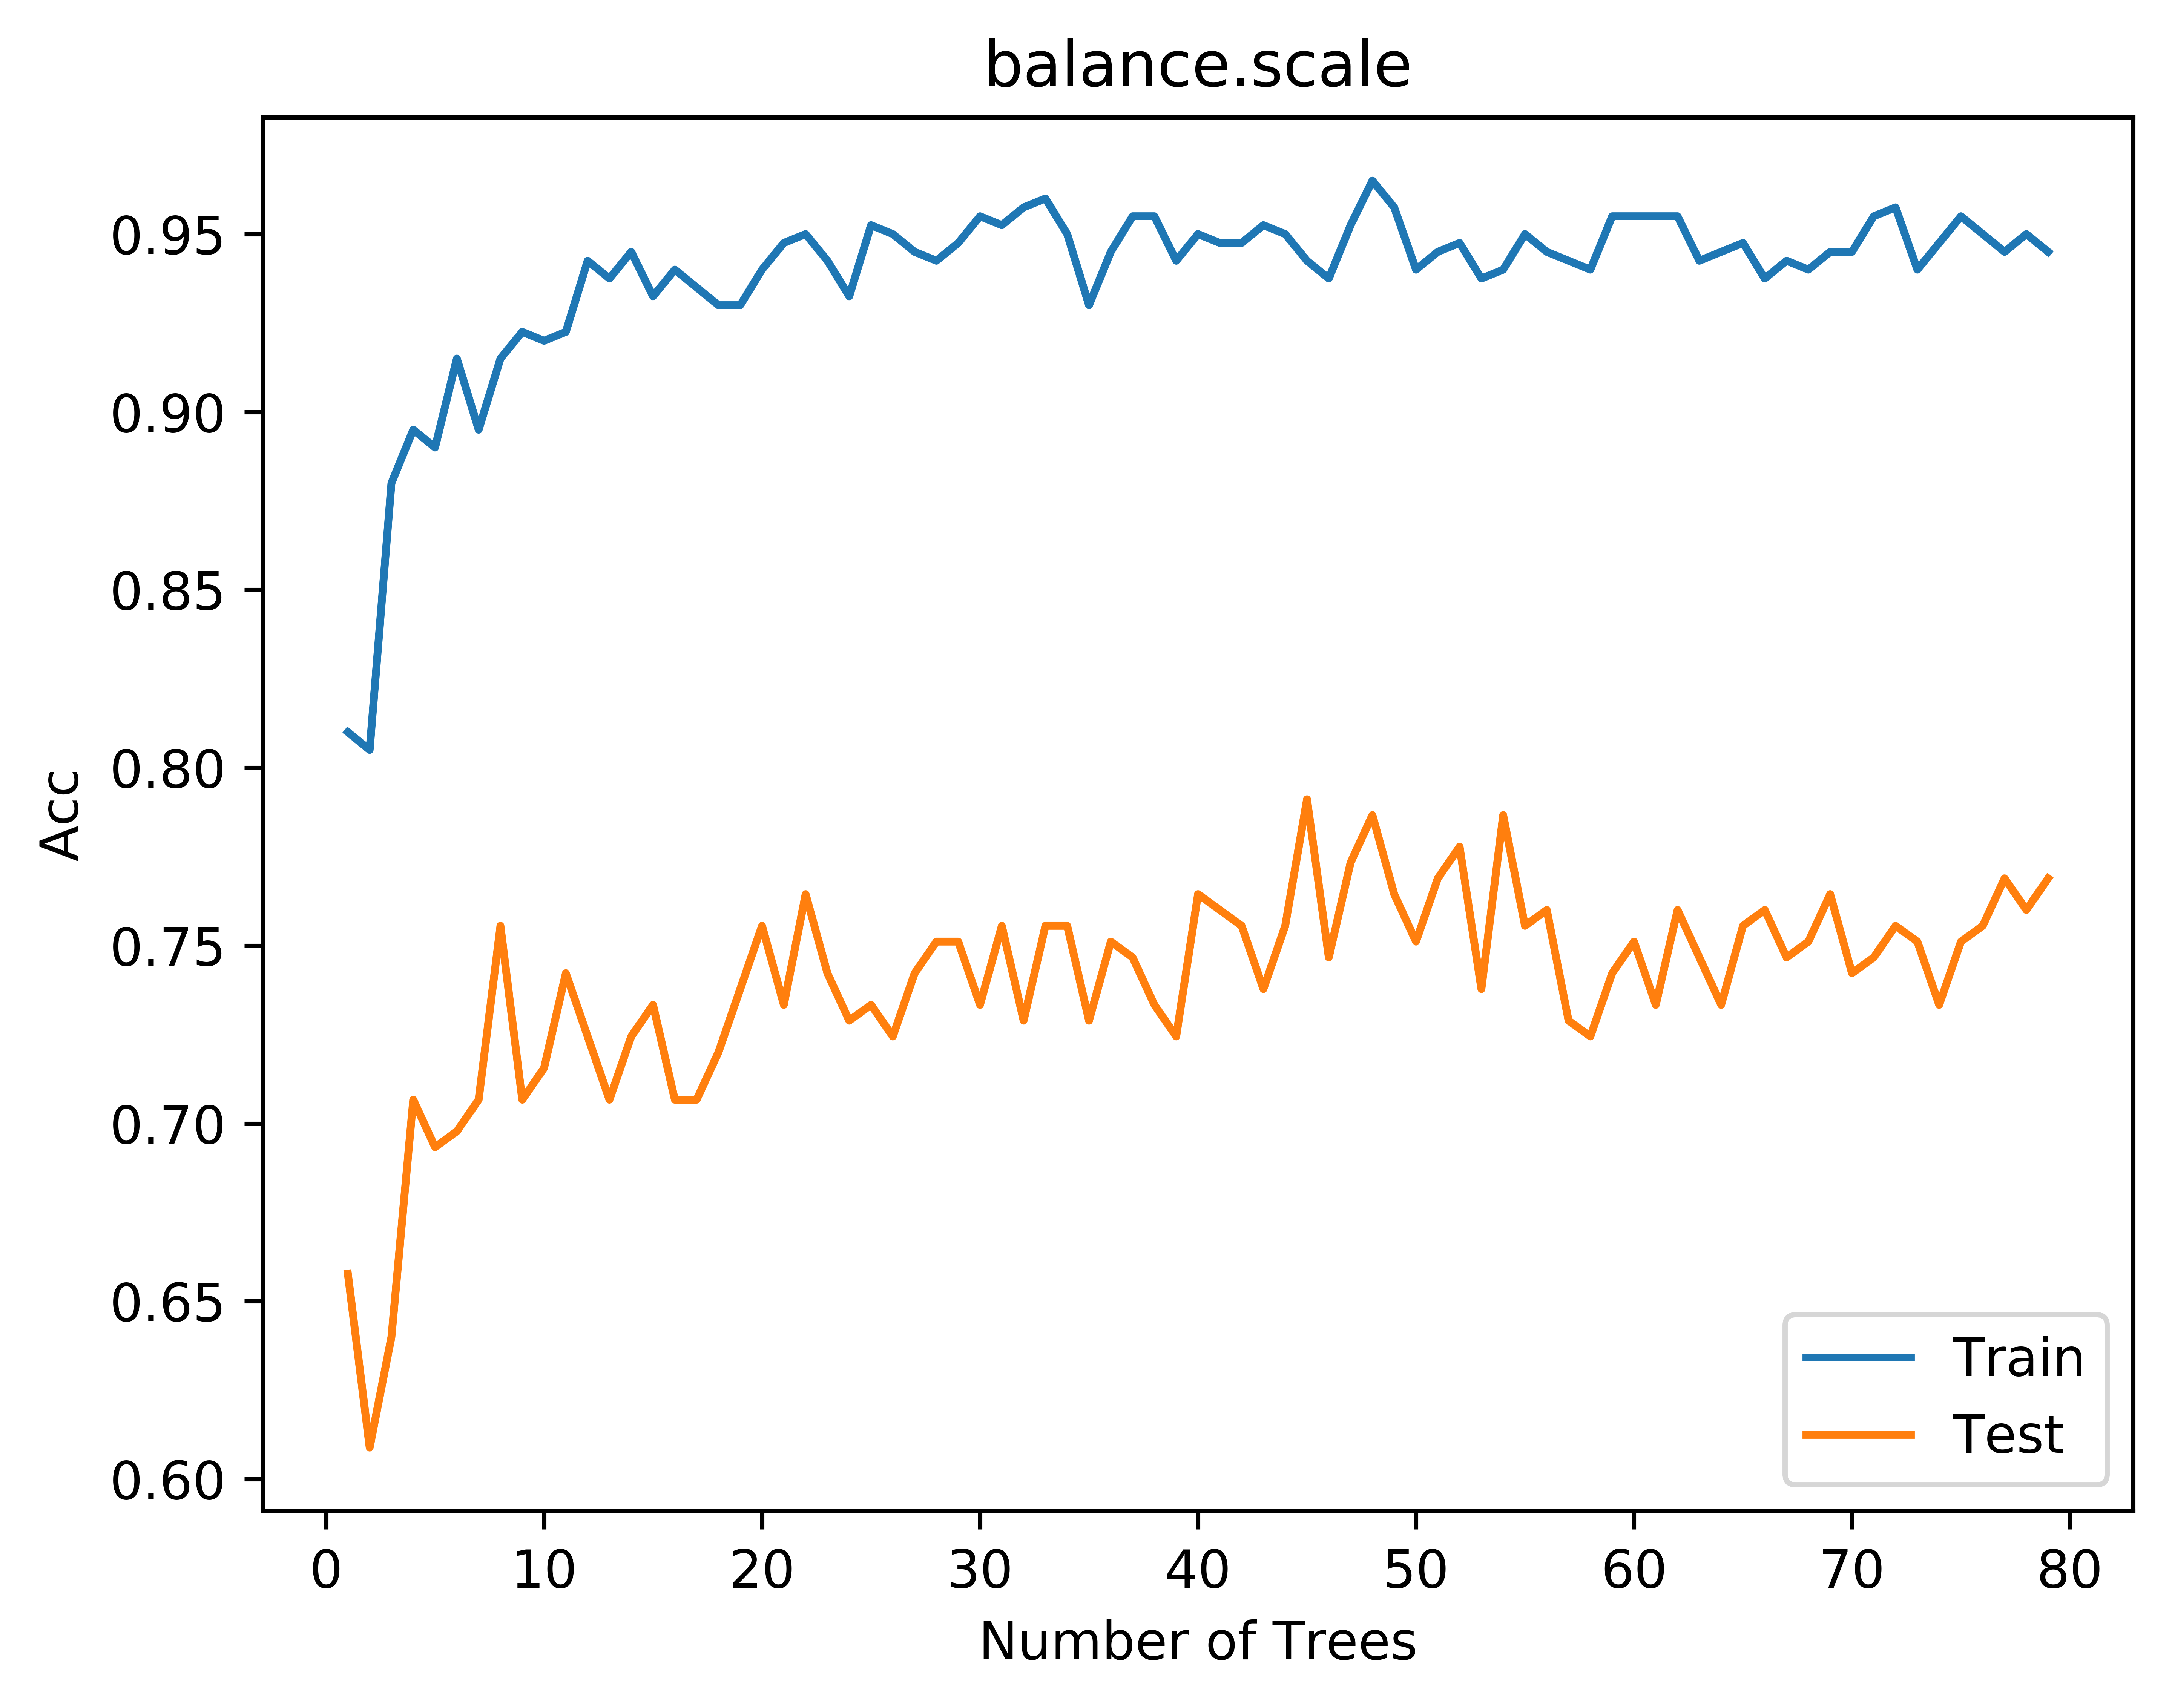
\includegraphics[width=8cm]{code/pics/balance_scale_RandomForest}
  		\end{center}
	\end{figure}
	\begin{figure}[H]
  		\begin{center}
  			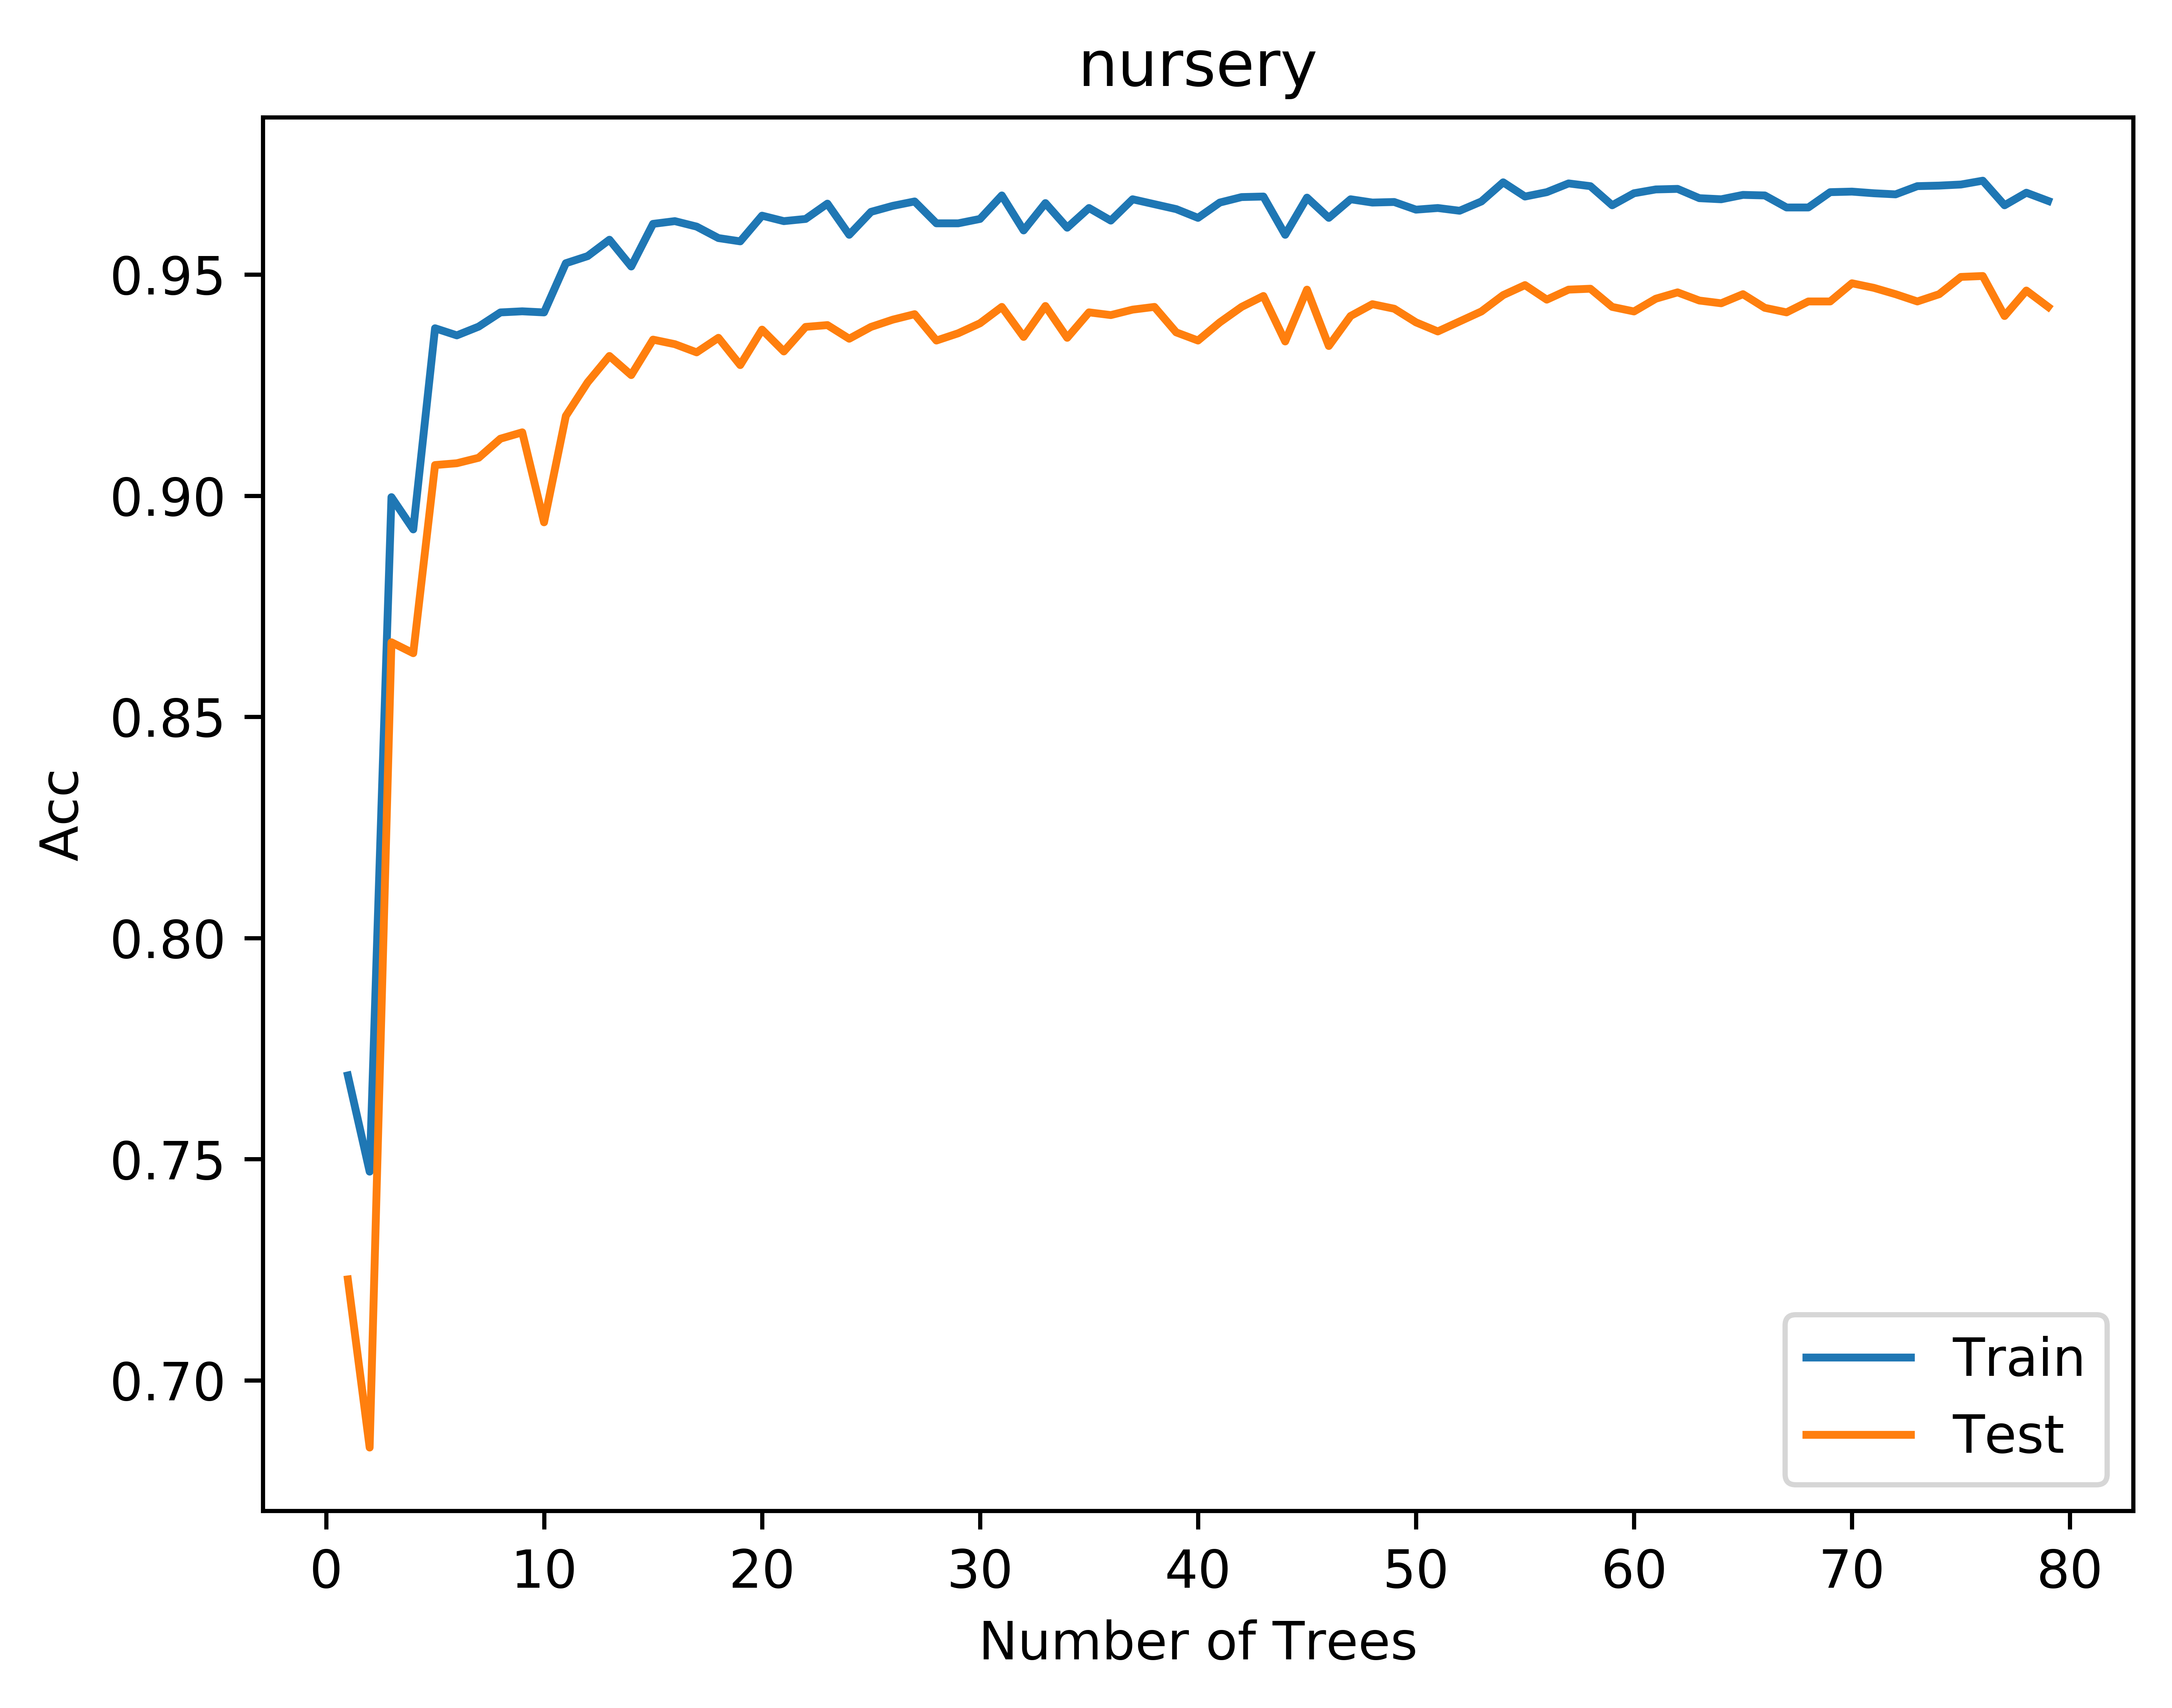
\includegraphics[width=8cm]{code/pics/nursery_RandomForest}
  		\end{center}
	\end{figure}
	\begin{figure}[H]
  		\begin{center}
  			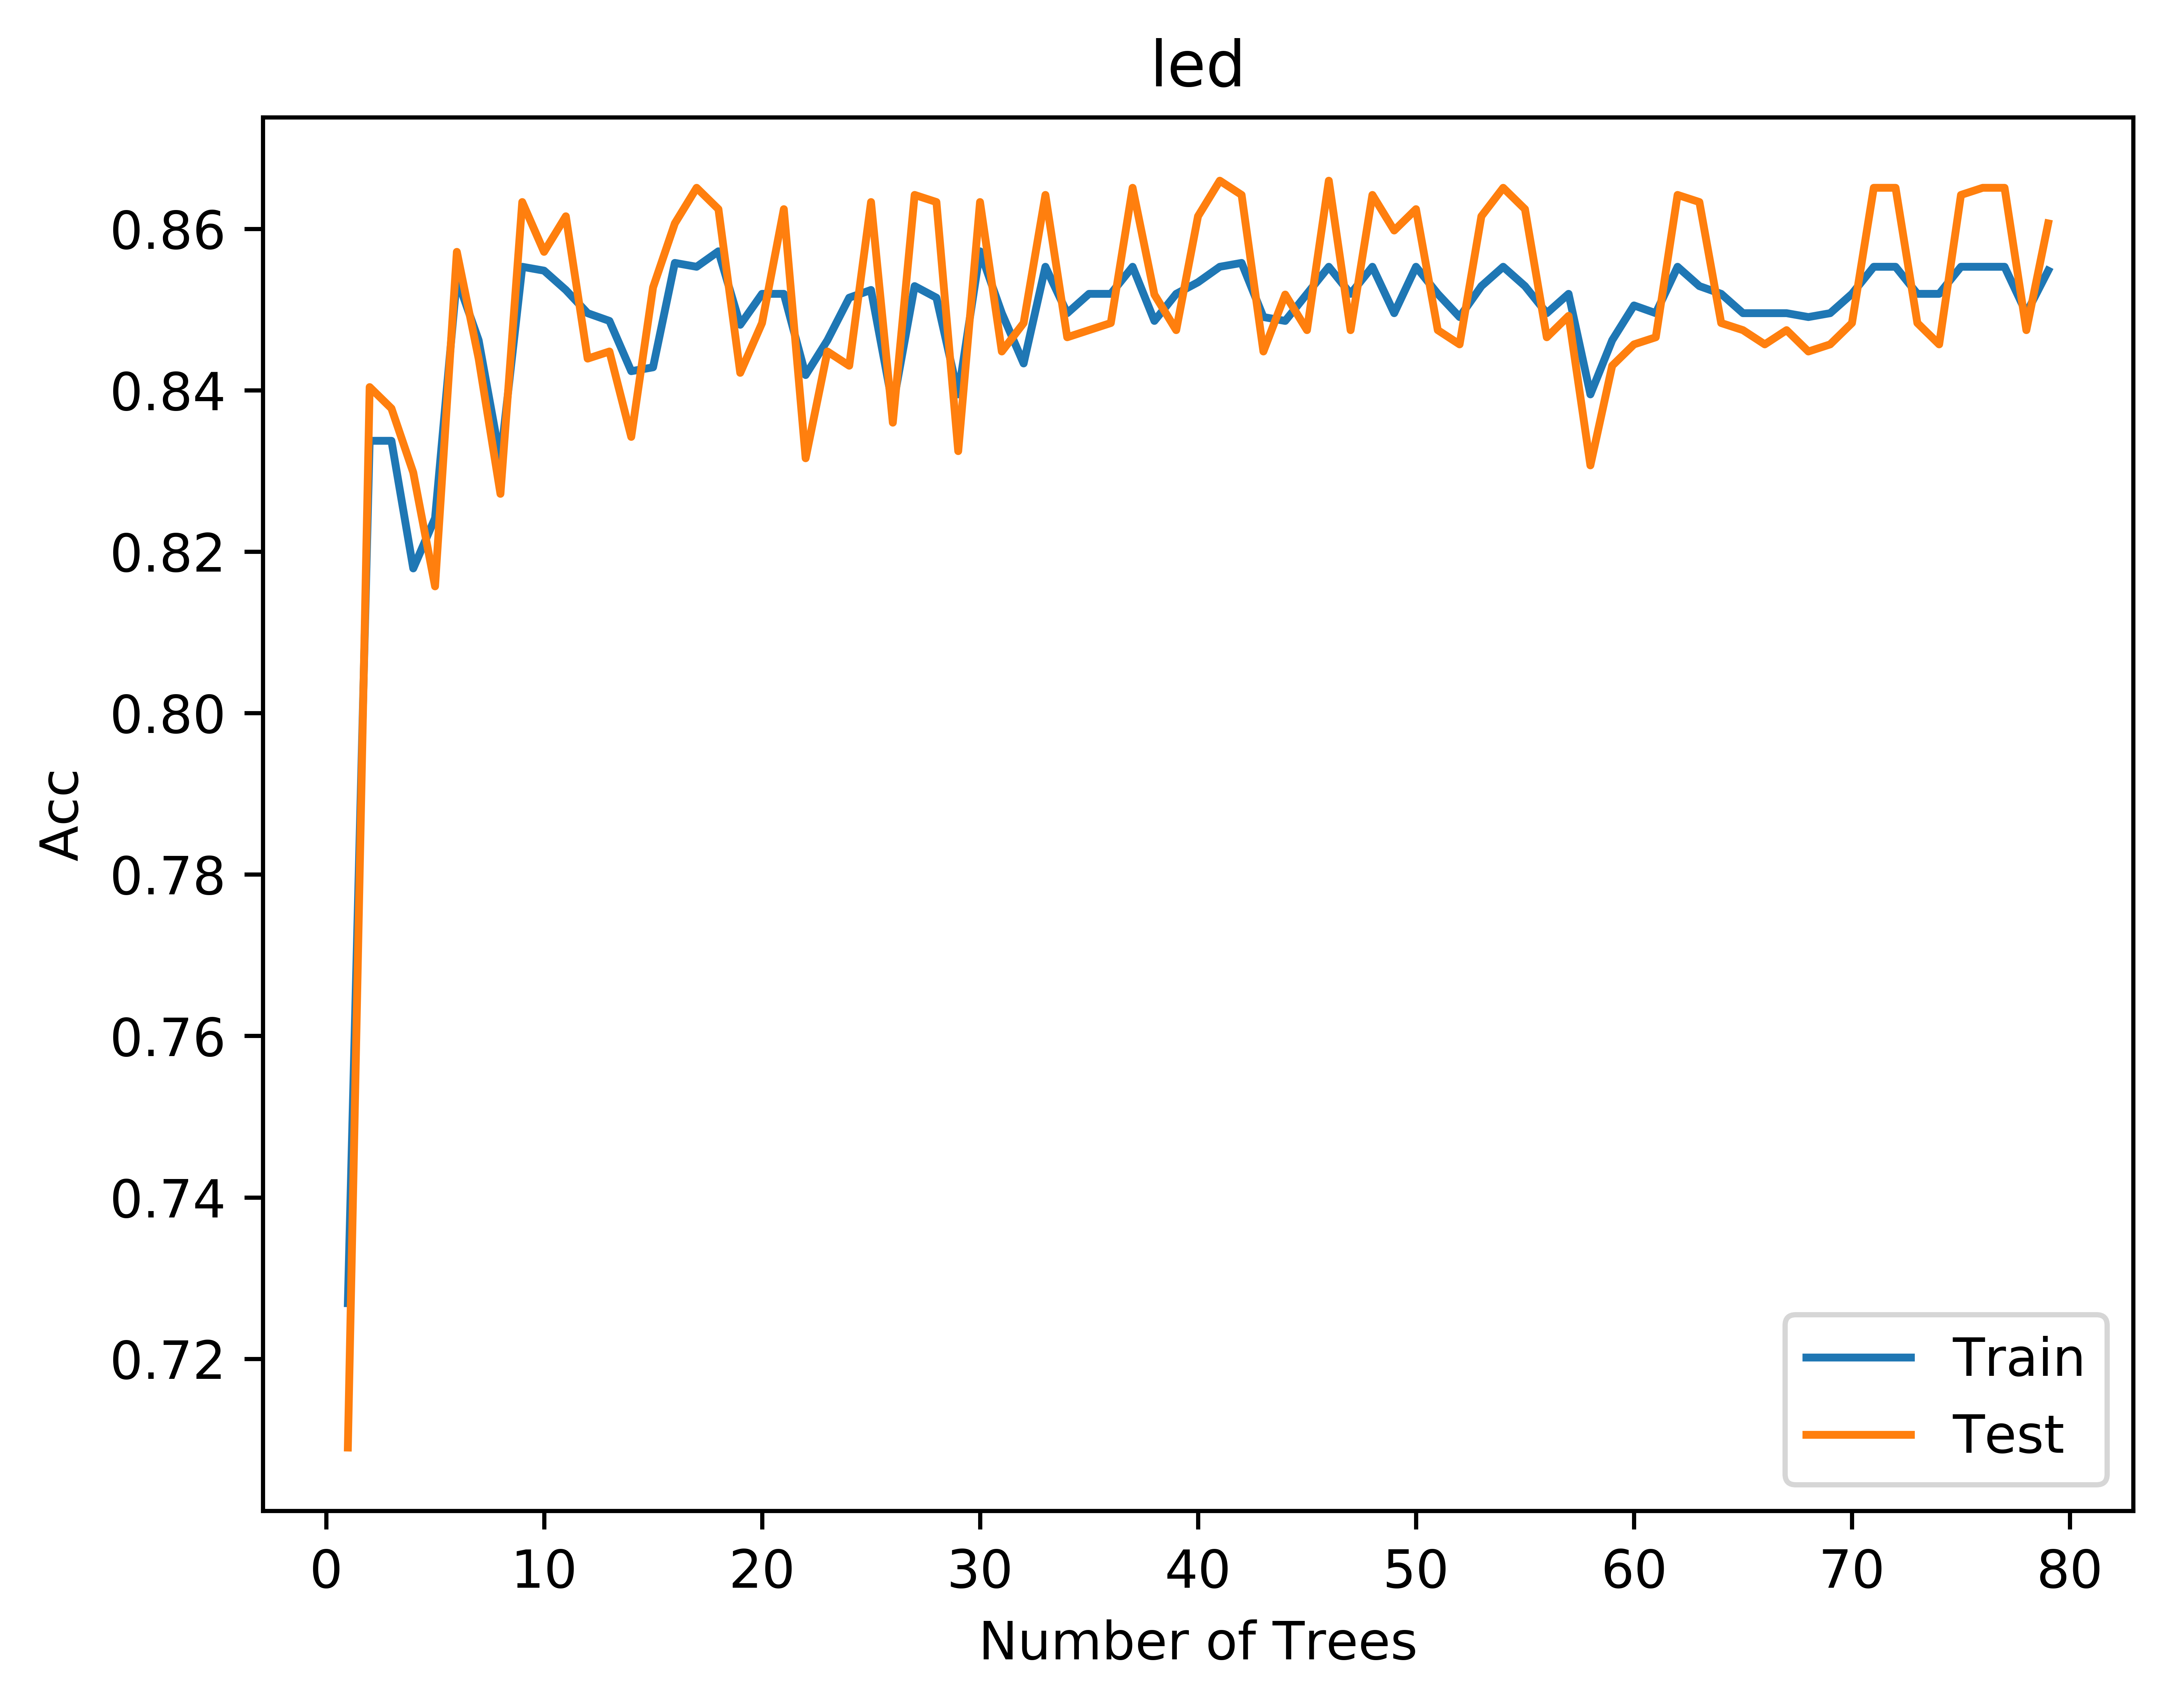
\includegraphics[width=8cm]{code/pics/led_RandomForest}
  		\end{center}
	\end{figure}
	\begin{figure}[H]
  		\begin{center}
  			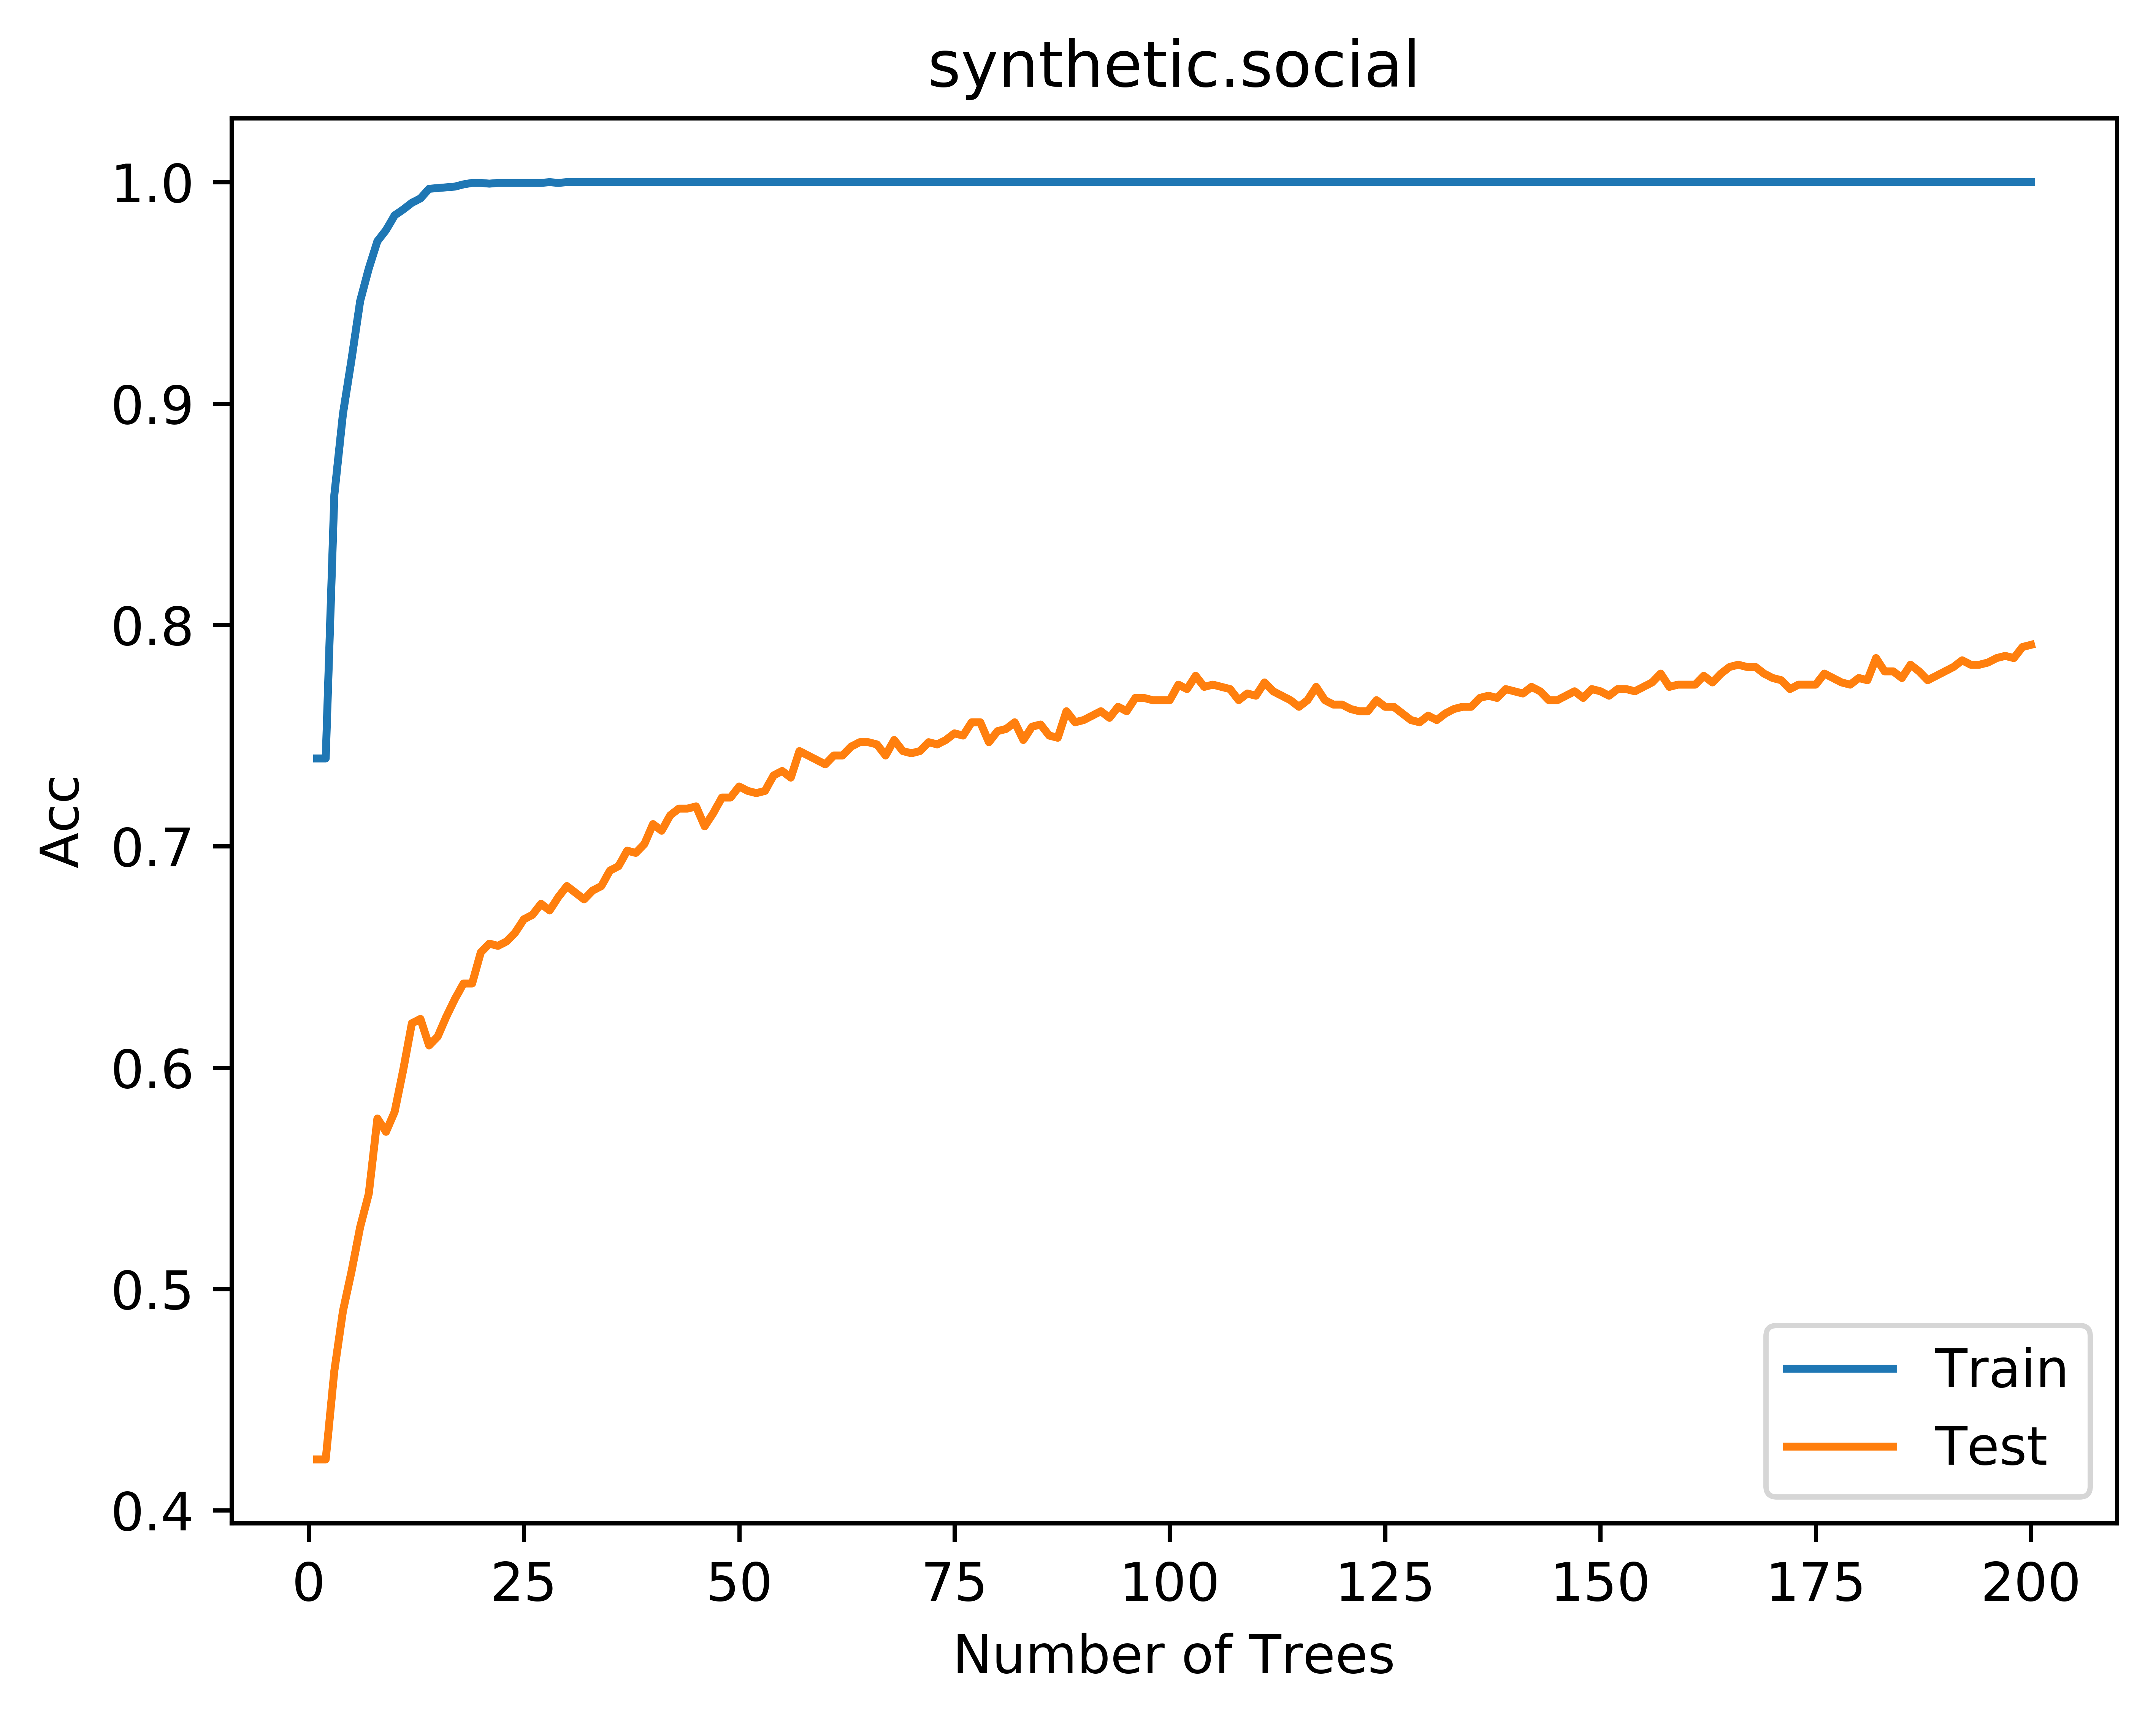
\includegraphics[width=8cm]{code/pics/synthetic_social_RandomForest}
  		\end{center}
	\end{figure}
	
	In order to save training time, we pick hyper-parameters that has least depth or number of trees possible while reaching the max accuracy, so that we choose:
	\begin{center}
		\begin{tabular}{|c | c | c |}
			\hline
			& Decision Tree (Depth) & Random Forest (Number)\\
			\hline
			\textit{balance.scale} & 4 & 45\\
			\hline
			\textit{nursery} & 8 & 42\\
			\hline
			\textit{led} & 7 & 20\\
			\hline
			\textit{synthetic.social} & 8 & 200\\
			\hline
		\end{tabular}
	\end{center}
	
	\section{Conclusion}
	\paragraph{}
	From the results above, we conclude that ensemble method improves the performance of the basic classification method by reducing the variance and increase the testing accuracy.
\end{document}